%!TEX root = ../dissertation.tex

\begin{savequote}[75mm]
Another inspiring quote for this chapter
\qauthor{Another author maybe}
\end{savequote}


\chapter[HPC in Healthcare: Business Model Transformations]{High-performance computing in healthcare: Identifying business model evolution via large language model and topic modeling}

\lettrine[lines=3]{\textcolor{SchoolColor}{T}}{his paper investigates the impact of}
technological advancements on the evolution of business models, with a specific focus on the healthcare sector. Manual analysis of business models from numerous financial reports poses significant challenges due to its time-consuming nature. To address this, our study introduces an automated framework
for business report analysis, leveraging advanced large language model
(LLM) and topic modeling techniques to explore how business models in healthcare evolve with High performance computing (HPC) adoption. This framework enables
the extraction and in-depth analysis of the business model from various reports,
uncovering a trend towards technology-driven and patient-centric models. It also identifies a shift toward recurring revenue models, diminishing
dependence on traditional funding sources like government contracts. Furthermore, our findings emphasize the growing significance of data and technological intellectual property in shaping the business landscape of healthcare. These insights highlight the substantial changes brought about by HPC in the business and economic landscapes of healthcare, providing valuable guidance for strategic planning and investment decisions. This analysis advocates for the enhanced integration of HPC technologies in the healthcare sector to fully leverage its potential for innovation and improved patient outcomes.



\section{Introduction}\label{sec1}

High-performance computing (HPC) has emerged as a pivotal technology in transforming the healthcare domain from a business perspective, enabling advancements in patient care, operational efficiencies, and innovation~\cite{belle2015big, veerla2023hpc}. HPC's role in healthcare extends from accelerating drug discovery and genome research to enhancing computational methods for large-scale data analysis, directly impacting the quality, speed, and cost-effectiveness of healthcare services~\cite{CHEN20181241,jumper2021highly,schmidt2017next}. The synergy between HPC and biomedical informatics accelerates the development of Artificial Intelligence (AI) methods, facilitating the development of advanced diagnostic tools and
personalized medicine approaches, tailoring treatments to individual patient
profiles, which were previously unattainable~\cite{bastrakov2013high,molidor2003new,lightbody2019review}. HPC��s role in advancing medical research cannot be over stated. It enables researchers to conduct complex simulations and analyses, leading to breakthroughs in understanding diseases and developing new treatments~\cite{ge2013molecular,kharche2008simulation,perrin2010model}. Moreover, the intersection of cloud computing with HPC introduces a paradigm shift in managing healthcare data, offering scalable and flexible solutions that enhance the quality and accessibility of care~\cite{hussein2013healthcare,lo2016mobile}. This integration facilitates systematic performance management and quality of care across the healthcare system, leveraging cloud technology for superior interoperability and data management~\cite{muhammed2018ubehealth,eze2016leveraging}. Additionally, the application of HPC for medical monitoring, particularly during pandemics, illustrates its essential role in supporting healthcare systems by ensuring the efficient and timely processing of medical data, which is vital for patient care and management~\cite{dananjayan2020artificial,majeed2021applications}.

The integration of HPC within the healthcare sector highlights its potential to drive business innovation. Investigating the business models of companies adopting HPC in healthcare offers valuable insights into the sector's business and economic dimensions, and provides a comprehensive understanding of the current landscape and potential future directions~\cite{reim2020implementation,muhtarouglu2013business}. Such insights can inform strategic planning and investment decisions within healthcare businesses utilizing HPC, identifying promising areas for further exploration and development. In this research, we applied the Business Model Canvas (BMC) framework by Osterwalder and Pigneur to examine companies' business models through detailed perspectives derived from their annual reports and conducted separate analyses~\cite{osterwalder2010business}. However, the vast number of companies updating their business reports annually, combined with rapid technological progress, challenges the manual analysis of BMC, making it both difficult and time-consuming. As a result,  there's a clear need for an automated tool that can effectively analyze a large volume of text, converting them into meaningful insights for business or strategic decision-making in the healthcare sector. We adopt recently developed topic modeling algorithms Top2Vec~\cite{angelov2020top2vec}, to manage extensive text collections and automatically uncover topics with significant keywords for easy understanding. By examining the evolution of companies' business models in the healthcare sector before and after implementing HPC from various perspectives, we gain insight into how HPC is accelerating business model innovation in the industry.

In this study, we develop an automatic business report analysis framework to invistigate how HPC impacts the business model evolution of companies in the healthcare domain. The primary contributions of this work are twofold:

\begin{enumerate}
\item We developed an automatic business model analysis framework, from business report retrieval and analysis to visualizations to depict business model evolution from different perspectives based on BMC. This adaptable pipeline can be generalized to other domains by modifying the business report retrieval rules.
\item By implementing an automated business model analysis framework, this study explores the transformation trends in business models among companies integrating HPC into healthcare. Our analysis reveals notable shifts: the healthcare sector is embracing AI, analytics, and cloud computing, moving towards technology-driven models. Firms have become more patient-focused, targeting diverse markets and prioritizing direct engagement. There is a move towards recurring revenue models, which lessens dependence on government contracts. Significantly, data and technological intellectual property have become key resources, surpassing traditional manufacturing and patents. These observations offer meaningful direction for upcoming investments and the strategic development of HPC in the healthcare industry, aiding in decision-making and resource allocation.
\end{enumerate}

\section{Theoretical Background}\label{sec2}
\subsection{Business model analysis and business model canvas}\label{subsec2.1}

The study of business models began to evolve as a distinct field, offering an alternative to conventional management methodologies in the mid-1990s~\cite{massa2017critical,zott2011business}. Business model is a conceptual framework that outlines how a company creates, delivers, and captures value. Teece et al. describe a business model as the architecture of value creation, detailing how a company delivers value to customers and converts it into profits~\cite{teece2010business}. This framework encompasses the mechanisms of value creation, delivery, and capture, reflecting management's hypothesis about customer needs and organizational capabilities to meet these needs profitably. Baden-Fuller and Haefliger~\cite{baden2013business} expand on this by defining the business model as a system for identifying the customer base, engaging with their needs, delivering satisfaction, and monetizing the value created, which is fundamental for linking technological innovation with firm.

While the term ``business model" is used frequently in academic and professional discourse, its interpretation diverges among scholars~\cite{al2010developing,sorrentino2015term,massa2017critical}. Despite the varied definitions, the essence of business models consistently emphasizes the importance of value creation. Fundamental to these models are the resources and operational activities involved~\cite{morris2005entrepreneur}. The variance in conceptualizations has led to many ontologies and methods for business modeling in academic research. Given our research's emphasis on analyzing business models from a systemic perspective, BMC serves as a prime example of this approach~\cite{kamprath2012systematic,upward2013towards}.


BMC originally conceptualized by Osterwalder and Pigneur~\cite{osterwalder2010business}, has emerged as a strategic management and entrepreneurial tool that allows organizations to describe, design, challenge, and pivot their business model. It has proven to be a comprehensive approach to business models and the effectiveness of the BMC in analyzing business models is well-documented across various studies and applications~\cite{muhtarouglu2013business,mustaniroh2020analysis,muller2019business}. The canvas encapsulates the essence of a business's operational blueprint across nine components, seamlessly interconnected to highlight how companies create, deliver, and capture value. These components include Value Propositions, outlining the problem solutions or needs fulfillment offered; Customer Segments, which delineates the target audience; Channels, indicating how a business reaches its customer segments; Customer Relationships, defining the nature of the interaction with customers; Revenue Streams, identifying the income sources from value propositions successfully delivered; Key Resources, highlighting the assets essential for operations; Key Activities, describing the most important actions a business must undertake; Key Partnerships, pointing out the network of suppliers and partners that make the business model work; and Cost Structure, detailing the monetary consequences of operating under a particular business model~\cite{osterwalder2010business}. Together, these elements provide a comprehensive snapshot, not only facilitating a deep understanding of a business's functioning core but also serving as a dynamic blueprint for innovation and strategic adjustment. This framework has not only been pivotal in aiding startups and established enterprises in navigating the complexities of their operations but has also fostered a universal language for discussing business models in a structured and coherent manner

\subsection{Topic modeling techniques }\label{subsec2.1}

Topic modeling, a branch of unsupervised machine learning, is designed to identify latent thematic structures within text corpora~\cite{blei2012probabilistic}. It classifies documents into topics based on the frequency and co-occurrence of words, serving as a critical tool for managing large, unstructured datasets and facilitating exploratory data analysis~\cite{jacobi2018quantitative}. Key techniques include Latent Dirichlet Allocation (LDA)~\cite{blei2003latent}, Non-negative Matrix Factorization (NMF)~\cite{lee1999learning}, and Latent Semantic Analysis (LSA)~\cite{deerwester1990indexing}, which are employed across text mining, information retrieval, and the digital humanities~\cite{alghamdi2015survey,huang2018analyst,yi2009comparative,meeks2012digital}. The utility of topic modeling extends to various fields such as marketing, healthcare, and social sciences, to detect trends within vast literature, social media content and reports ~\cite{amado2018research,karas2022experiments,sarioglu2013topic}. LDA is arguably one of the most widely used algorithms for topic modeling. Despite its popularity, LDA faces challenges like data preprocessing and the difficulty of interpreting topics~\cite{maier2018applying,angelov2020top2vec}, leading to the exploration of alternatives like entity linking (EL)~\cite{10.1145/3126686.3126776}. Recent advancements have introduced deep learning techniques like Top2Vec~\cite{angelov2020top2vec}, which leverage doc2vec models to generate semantic vector representations of words, thereby enhancing topic identification and creating integrated vectors for topics, documents, and words. Comparative studies suggest Top2Vec often outperforms LDA in quality of results~\cite{egger2022topic,karas2022experiments}.

\section{Materials and methods}\label{sec2}

In this section, we offer a detailed overview of the data and analytical methodology utilized in our study. Figure~\ref{fig:5-1} presents the automated literature review framework, comprising four key phases: business report retrieval and extraction, BMC extraction, topic modeling, and visualization. Detailed descriptions of each phase are provided in the following subsections.

\begin{figure}[!h]
\centering
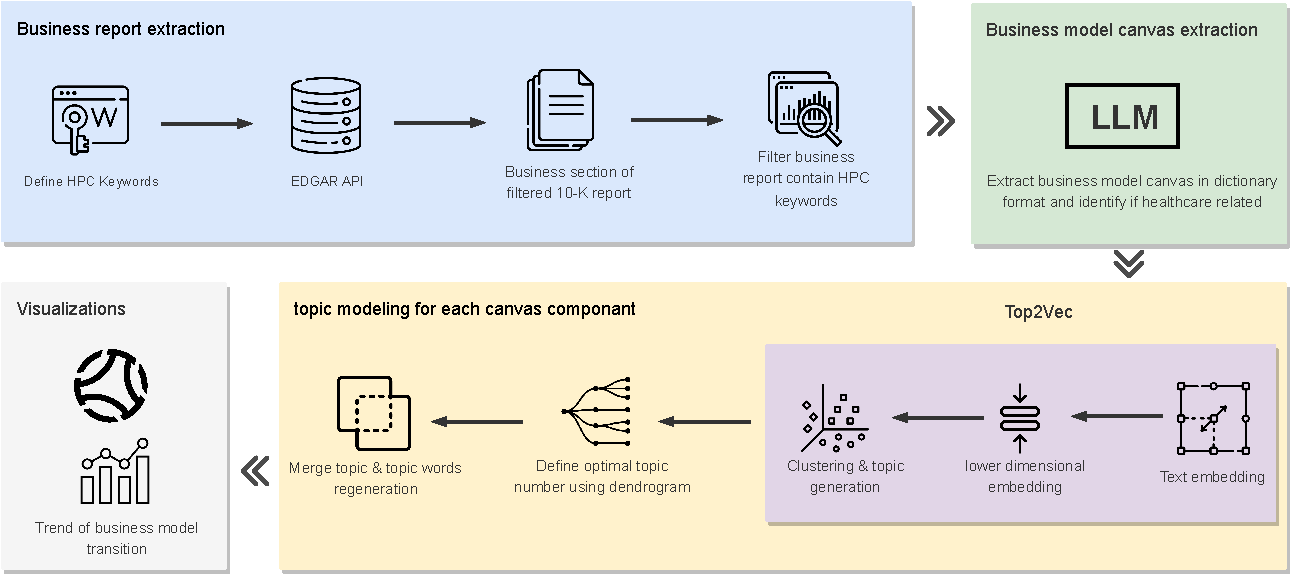
\includegraphics[width=0.95\textwidth]{5-1.pdf}
\caption{Automatic literature review pipeline consists of four stages: business report retrieval and extraction, BMC extraction, topic modeling, and visualization}
\label{fig:5-1}
\end{figure}

\subsection{Business report retrieval and extraction}\label{subsec2.1}
\subsubsection{Data source}\label{subsubsec2.1.1}

We propose to use the 10-K annual report in the analysis process. These reports are required by the U.S. Securities and Exchange Commission (SEC) for all publicly traded companies within the United States, serving as a comprehensive disclosure of their business operations and financial outcomes over the fiscal year\footnote{\url{https://www.sec.gov/files/form10-k.pdf}}. Public companies with significant assets are required to file these reports annually, contributing to a vast repository of over ten thousand documents available to the public. These documents are made publicly accessible through the Electronic Data Gathering, Analysis, and Retrieval (EDGAR) online database\footnote{\url{http://edgar.sec.gov}}, allowing for direct access via the EDGAR system's API\footnote{\url{https://www.sec.gov/edgar/sec-api-documentation}}. Given that the general filing deadline for 10-K reports is 90 days after the end of the fiscal year, and considering the timing of our research, filings for the year 2023 may not be fully complete. To guarantee the comprehensive collection of reports, we have limited our extraction to include filings up until the year 2022.

Each 10-K report is structured into 15 Items. The SEC's guidelines stress the significance of the description of business in Item 1 of the financial reports, which is of great interest for our research~\cite{securities2020modernization}. The guidance emphasizes the inclusion of pivotal aspects of a company's trajectory, such as historical development, strategic shifts, and current operational landscape. This information serves as a foundation for analyzing business models as it offers essential insights into various dimensions of the company's activities and intentions. Understanding the general development of the business, including detailed disclosures regarding revenue-generating activities, product development efforts, resource utilization, and regulatory compliance, illuminates the company's core operations and competitive positioning. In essence, the Item 1 section acts as a comprehensive narrative, providing vital context and insights crucial for understanding the company's strategic direction and competitive dynamics.

\subsubsection{HPC related business report retrieval pipeline}\label{subsubsec2.1.3}

We develop an automated pipeline for report retrieval and query expansion using the EDGAR API, initiating with the identification of HPC keywords, including `high performance computing', `supercomputing', and `cloud computing'. This initial set is iteratively expanded by incorporating additional relevant keywords derived from the reports, enabled through a keyword frequency analysis. Terms associated with HPC, appearing more than 50 times and not initially included, are added to the query. This method of automatic query expansion incorporates HPC-related synonyms and terms, such as `high-performance computing', `high performance computer', `supercomputer', `HPC cloud', `cloud services', and `cloud platform'. This process continues until no new significant keywords emerge, ensuring comprehensive coverage of the search area. Business reports identified through this refined search are then prepared for the subsequent analysis.

\subsection{Business model canvas extraction}\label{subsec2.2}

The business section of 10-K reports extracted in our study varies significantly in length, ranging from 1066 to 40406 words with an average word count of 6453, with key information pertaining to a company's BMC often concealed within the text. Applying topic modeling directly to extensive texts in thousands of documents does not effectively reveal transitions between different business model perspectives. Moreover, this approach lowers the analysis quality, as irrelevant text obscures essential keywords, complicating interpretation. Consequently, extracting information relevant to the nine components of the BMC becomes essential for a more targeted topic modeling process. However, manually reviewing hundreds of reports to construct a BMC for each is prohibitively time-consuming. Recent advances in large language models (LLMs) have demonstrated their effectiveness in zero-shot information extraction tasks, as highlighted by studies employing the GPT series models~\cite{kartchner2023zero,wei2023zero,hu2024zero}. Leveraging this advancement, we have designed prompts tailored for GPT-3.5 (\texttt{gpt-3.5-turbo-1106}) and GPT-4 (\texttt{gpt-4-1106-preview}) APIs\footnote{\url{https://platform.openai.com/docs/models/overview}},  chosen based on the length of the input text, to systematically extract the BMC from 10-K reports. the prompts are available at a public GitHub
repository\footnote{\url{https://github.com/tuohai1992/Business-model-canvas-topic-modeling/blob/main/Business_model_canvas_extraction_prompt.py}}. The outputs are organized in a format of python dictionary, detailing the nine essential components of the BMC. An example of this method is depicted in Figure~\ref{fig:5-2}, which presents the BMC extracted from the business section of Advanced Micro Devices (AMD)'s 10-K report, illustrating the GPT models' capacity to accurately identify and organize relevant information into the canvas structure.

\begin{figure}[!h]
\centering

\includegraphics[width=0.95\textwidth]{5-2.png}
\caption{Example of business model canvas extracted by GPT-3.5 in a format of python dictionary}
\label{fig:5-2}
\end{figure}

\subsection{Identify healthcare related business model canvas}\label{subsec2.3}

Unlike extracting HPC-related business reports using specific HPC terminology, identifying keywords related to healthcare presents a broader and more generalized challenge. The determination of a company's involvement in the healthcare sector heavily relies on the semantic context. For example, references to `high performance computing' alongside `health' or `healthcare' in some business reports often pertain to system health, such as fault tolerance, job scheduling, and interconnection, rather than human health. The Standard Industrial Classification (SIC) Codes in a company's EDGAR filings are intended to identify its primary business line. However, despite many companies operating in multiple business lines, only one SIC code is assigned to each company in EDGAR filings. Consequently, filtering companies by SIC code may exclude many that are involved in healthcare but not as their primary business. Therefore, we utilize the GPT-4 model for detecting non-healthcare-related BMCs. Similar to studies~\cite{carpenter2023using,bommarito2022gpt}, we design prompts for the gpt-4-1106-preview API to evaluate the relevance of BMCs extract from 10-K reports to the healthcare sector, classifying them as either healthcare-related or non-healthcare-related for subsequent analysis. The prompts are also available at our public GitHub repository\footnote{\url{https://github.com/tuohai1992/Business-model-canvas-topic-modeling/blob/main/Dentify\_healthcare\_related\_business\_model\_canvas\_prompt.py}}.

To evaluate the effectiveness of the GPT-4 model in identifying healthcare-related 10-K reports, we extract 19 SIC Codes associated with healthcare from the SEC.gov database. Using these codes, 277 healthcare-related 10-K reports across 51 companies been located. We then input the BMC extracted from these 277 reports into the GPT-4 model to determine their relevance to healthcare. Our analysis compares GPT-4's classification results with those based on the SIC codes, uncovering 13 inconsistencies. A detailed review indicates that the SIC codes have misclassified 12 reports as being healthcare-related, whereas GPT-4 inaccurately identifies one report as unrelated. After excluding reports with incorrect SIC codes, GPT-4's accuracy in classifying healthcare-related 10-K reports improves to 99\%. Detailed validation approaches are elaborated upon in the Appendix (section A.1).

To analyze the transition in the business model of companies engaged in the healthcare sector before and after adopting HPC, we extract the BMCs from all historical 10-K reports of companies that had adopted HPC in their healthcare-related business during specific years. To prepare for the subsequent topic modeling, for each company, we select one BMC associated with both HPC and healthcare as the post-HPC adoption input and another BMC related solely to healthcare, serving as the pre-HPC adoption input. If a company's reports from multiple years are found to be related to both HPC and healthcare, we choose the most recent report and its corresponding extracted BMC. If a company's reports from multiple years are related solely to healthcare, we select the report from the median year along with its corresponding extracted BMC. This method is specifically designed to allocate several years to demonstrate a clearer evolution of the business model.

\subsection{Topic Modeling }\label{subsec2.4}
\subsubsection{Algorithm choice}\label{subsubsec2.4.1}

In this study, we applied the Top2Vec model, a novel approach to unsupervised learning within the realm of topic modeling~\cite{angelov2020top2vec}. Top2Vec stands out by combining word embeddings, dimensionality reduction, and density-based clustering to facilitate the automatic identification of topics and document embeddings, eliminating the need for pre-existing knowledge or human input. The process begins with the conversion of documents into dense vector representations through the doc2vec embedding algorithm~\cite{le2014distributed}. This technique effectively captures the semantic essence of texts, including contextual word usage, by representing them as vectors in a high-dimensional space. Documents that share semantic similarities are placed closer together in this space, indicating their relatedness. The algorithm then proceeds with dimensionality reduction using the UMAP technique~\cite{mcinnes1802umap}, a method rooted in manifold learning that adeptly conserves the integrity of both immediate and extensive data structures. This ensures a coherent representation in a compacted dimensional space, where emergent clusters of document vectors indicate separate topics.

The subsequent phase involves applying Hierarchical Density-Based Spatial Clustering of Applications with Noise (HDBSCAN), a density-based clustering algorithm, to discern these clusters~\cite{campello2013density}. HDBSCAN identifies regions of higher density in the document vector space and categorizing them into clusters. Each cluster, indicative of a unique topic, is characterized by a 'topic vector' �� a centroid that encapsulates the semantic essence of the topic. These topic vectors are then transformed back into the word space to construct interpretable topics, identifying keywords that closely align with each topic vector. 

\subsubsection{Identify optimal topic number using dendrogram and Topic merging}\label{subsubsec2.4.2}

In our initial assessment of the Top2Vec model outputs, utilizing Agglomerative hierarchical clustering to gauge topic similarity, we noticed a considerable overlap and an unnecessary level of detail among some topics.  For instance, an early review focusing on the cost structure aspect highlighted recurring discussions about training new employees and manufacturing costs, as indicated in the red boxes of Figure~\ref{fig:5-3}. We merge these overlapping topics, establishing nine as the ideal number of topics for modeling the cost structure. We applied a similar process to determine the optimal topic count for other BMC perspectives. By consolidating similar topics, we aim to achieve a more comprehensive understanding of business model evolution.

Agglomerative hierarchical clustering, enhanced by dendrogram visualizations, is a strategy for grouping similar elements based on their proximity~\cite{nielsen2016hierarchical}. This method begins with each element as a separate cluster and gradually merges them based on their similarity. We utilized cosine distance to measure the proximity between topic vectors, which is particularly effective for high-dimensional data like semantic word embeddings~\cite{orkphol2019word,rozado2019using}. This measure considers both the magnitude and orientation of the vectors, providing a more robust comparison than traditional methods like Euclidean distance, which only considers magnitude. In the context of our hierarchical clustering, we have adopted the average linkage method~\cite{nielsen2016hierarchical}. This clustering process results in a dendrogram that visualizes the relationships between topics in a hierarchical manner. The dendrogram helps in choosing where to cut the clusters to determine an optimal number of topics by showing how clusters merge at various levels of similarity. This visualization and the hierarchical clustering method offer a detailed view of the topic structure and connections, aiding in the selection of a suitable number of topics for further analysis.

Following the identification of the optimal topic count through dendrogram analysis, the next step involves consolidate topics. The Top2Vec algorithm features a hierarchical topic reduction function \texttt{hierarchical\_topic\_reduction} aimed at minimizing the topic count by iteratively merging the smallest topics with the most similar ones until a pre-set target is achieved\footnote{\url{https://github.com/ddangelov/Top2Vec}}. However, this method, which merges topics based on size rather than similarity, potentially overlooking emerging or distinct topics that could be of interest. Therefore, we suggest an alternative approach that emphasizes merging topics based on their similarity rather than size, in line with agglomerative hierarchical clustering principles. This method aims to maintain the relevance and distinctiveness of topics, thereby ensuring a more accurate and insightful analysis. 

\begin{figure}[!h]
\centering
\includegraphics[width=0.95\textwidth]{5-3.eps}
\caption{Dendrogram of hierarchical clustering with Identified optimal topic number (cost structure perspective)}
\label{fig:5-3}
\end{figure}

\subsection{Visualization }\label{subsec2.5}

We utilize two types of visualizations in our study. The first type includes classic area and line charts, which we used to depict the absolute numbers of health and HPC-related 10-K reports over the years, as well as their proportions relative to the total number of 10-K reports filed each year. This approach allows us to clearly observe the overall trend of HPC adoption within the healthcare industry. Secondly, to examine the transition in business models of companies in the health sector before and after the adoption of HPC, we employ chord diagrams for our visualizations. Chord diagram illustrates complex many-to-many relationships between entities using curved arcs within a circle, effectively revealing underlying patterns and trends~\cite{finnegan2019using}. This method enhances our understanding by visually representing the topic transitions within each component of the BMC for companies engaged in health-related businesses, both pre- and post-HPC adoption.

To generate chord diagrams, we constructed transition matrices that illustrate the shifts in company topics before and after HPC adoption for each BMC perspective. An example of how we built a topic transition matrix for the value proposition perspective can be found in section A.2 of the Appendix. We used PlotAPI\footnote{\url{https://plotapi.com/docs/visualizations/chord/}} in python for generating interactive chord diagrams, which are described here through static screenshots to depict their interactive capabilities. A chord diagram is a circular representation of interconnected data, where topics are depicted along the arcs and the connections between topics are shown as chords. Each arc represents the transition from one topic to another and the arc's thickness reflects the significance of the flow. In each chord diagram, we employ directed chords with arrows to signify the direction of a relationship. The topic indicated by the arrow denotes the topic of a particular BMC perspective categorized post HPC adoption, while the origin of the arrow indicates the topic of a BMC perspective categorized pre HPC adoption within the business. Additionally, to quantify transitional trends, we compute the number of reports categorized under specific topics before and after HPC adoption, subsequently calculating floating ratios for interpretation. 

\section{Results}\label{sec3}

In the results section, we first visualize the trends in the absolute number of HPC and healthcare-related 10-K reports over the years, as well as their ratio to the total number of 10-K reports. This visualization aims to illustrate the overall trend of HPC adoption in the healthcare industry. Subsequently, we employ interactive chord diagrams to depict the transition of each BMC perspective. These diagrams visualize the evolution of topics among companies engaged in health-related businesses both before and after the adoption of HPC. While analyzing the topic modeling outcomes across various perspectives, we identified clear trends of transition within the six dimensions: value proposition, customer segment, revenue stream, cost structure, key activities, and key resources. Furthermore, given the significance of the Value Proposition within the BMC, as it delineates the business's functions, addresses the problems it solves, and highlights its unique selling points in comparison to competitors. we delve deeper into this perspective by visualizing its emerging trends over time. We detail these observations within the results section and include an extensive chord diagram covering all BMC perspectives in the Appendix (section A.3).

\subsection{Overall trend of HPC adoption in healthcare business}\label{subsec3.1}

As shown in Figure~\ref{fig:5-4}, the adoption of HPC in healthcare-related businesses has experienced significant growth over the past two decades. The pace of growth has accelerated since 2008, corresponding to the remarkable advancements in supercomputing power during that period. In 2008, the PetaFlop barrier was surpassed, leading to exponential growth in computing power thereafter~\cite{grice2009breaking}. This has provided substantial support for complex simulations and the training of deep learning models in healthcare.

\begin{figure}[!h]
\centering
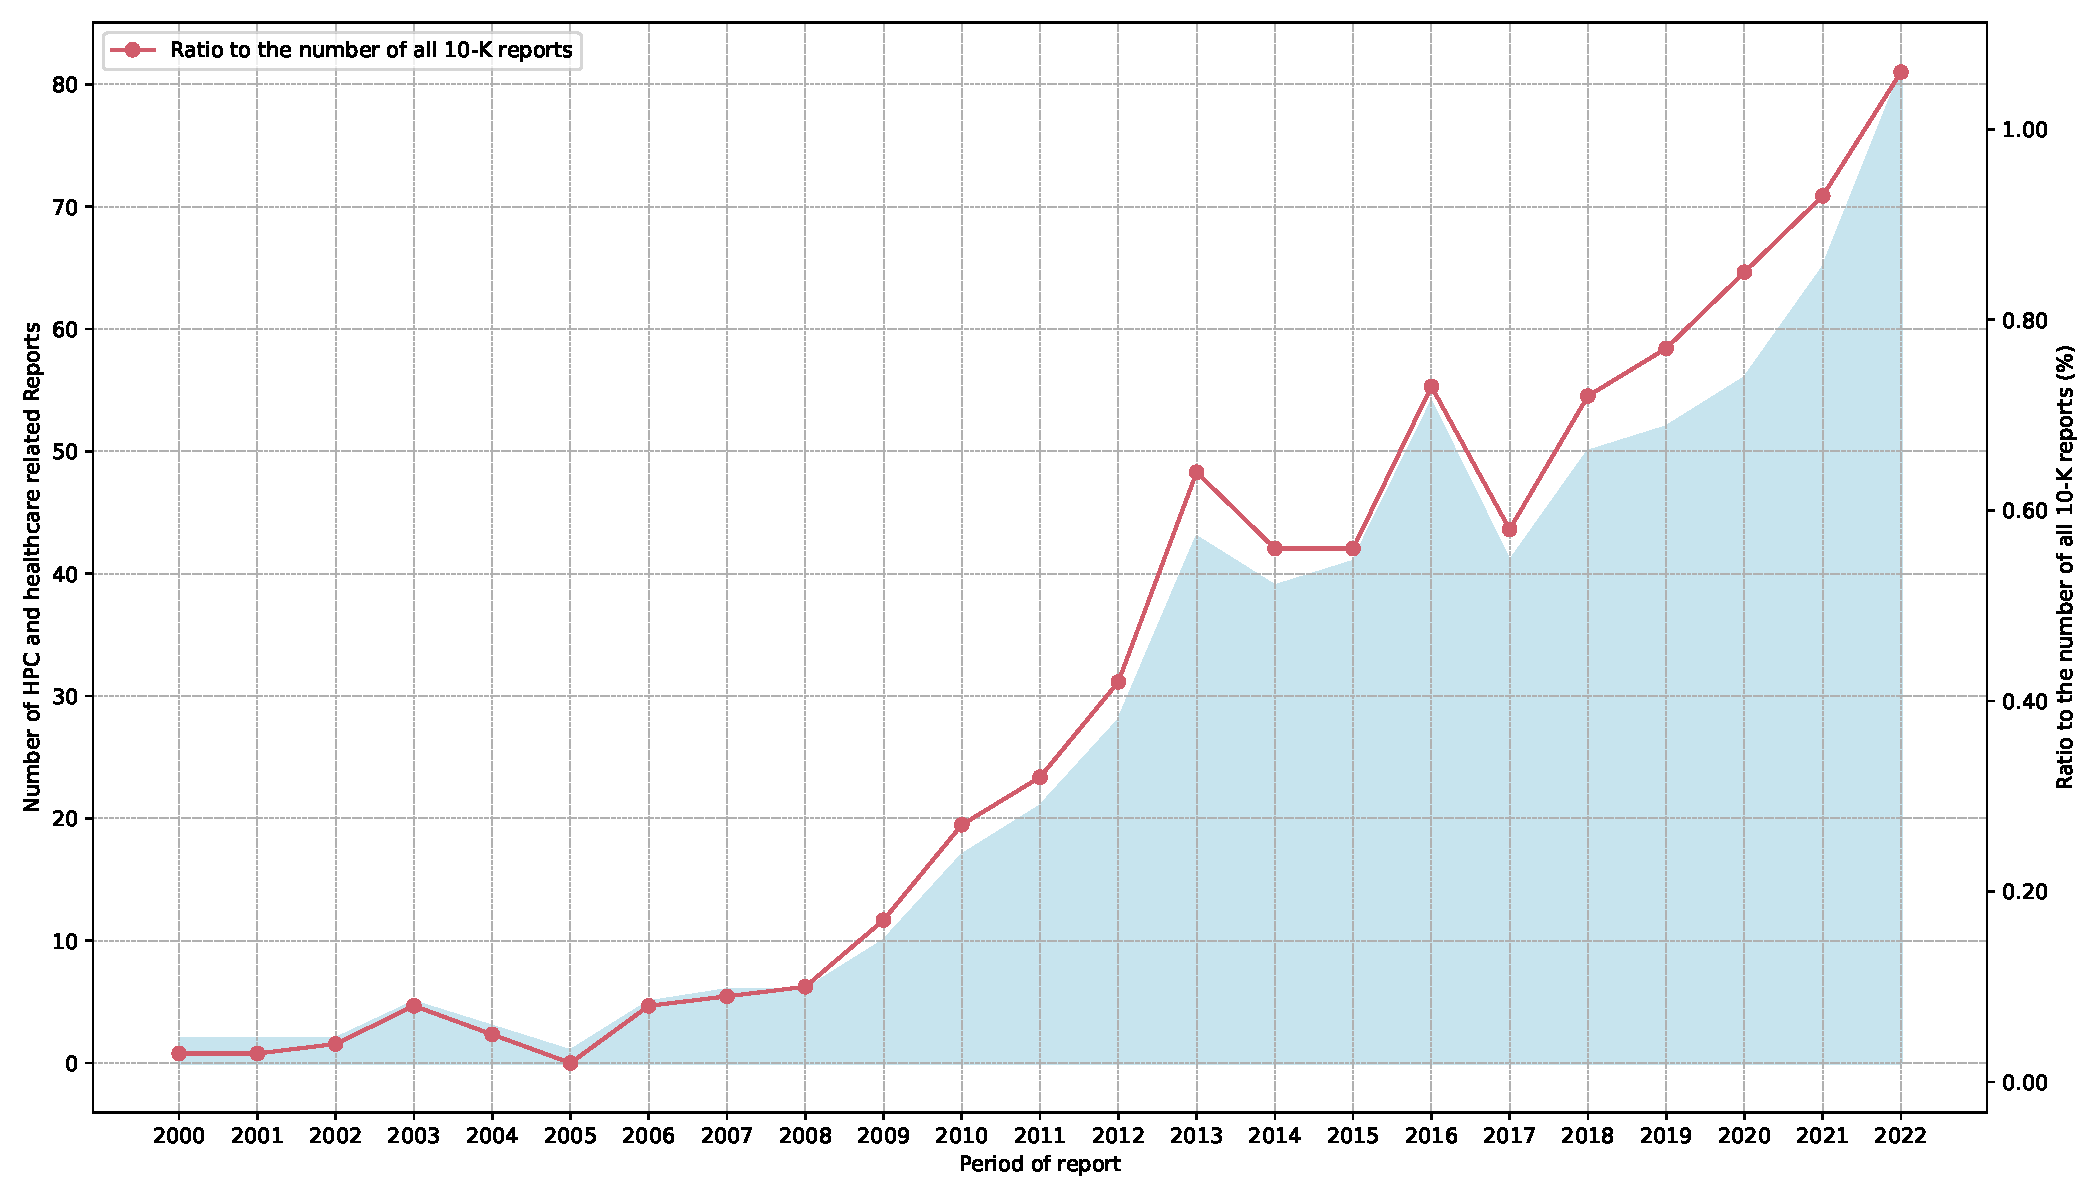
\includegraphics[width=0.95\textwidth]{5-4.pdf}
\caption{Absolute number of  HPC and healthcare-related 10-K reports according to years and also the ratio to the number of all 10-K reports filled that year}
\label{fig:5-4}
\end{figure}

\subsection{Value proposition transition}\label{subsec3.2}
\subsubsection{Value proposition transition pre- and post-HPC adoption}\label{subsec3.2.1}

The adoption of HPC by companies in the healthcare sector has brought a significant transition in terms of value proposition. The largest share of value propositions remains deeply rooted in the medical and clinical segment, underscoring a steadfast commitment to core healthcare services. However, there's a notable shift toward embracing cutting-edge technologies, evidenced by an 88\% increase in companies extending their operations into the data analytics and AI domains (panel (a) of Figure~\ref{fig:5-5}). The floating ratio is computed by subtracting the number of companies in specific topics before and after HPC adoption, then dividing by the number of companies before HPC adoption, based on the transition matrix. Section A.2 of the Appendix presents an example of a transition matrix from the value proposition perspective and illustrates how the chord diagram and floating ratios are generated based on it. This transition suggests an industry-wide recognition of the transformative potential of data-driven insights and in enhancing patient care and operational efficiency. To validate our observations, we examined the 10-K report of specific companies that underwent this transition. For instance, NEXTGEN HEALTHCARE, INC. (CIK: 708818), which demonstrated a shift from a clinically focused value proposition to business driven by data analytics.  Our analysis revealed that before 2009, NEXTGEN primarily developed and marketed healthcare information systems for physicians, hospitals, community health centers, and medical and dental schools. From 2009 onwards, after introducing web-based Software as a Service (SaaS) solutions for medical and dental practices, NEXTGEN pivoted to providing cloud-based healthcare technology solutions across the U.S. healthcare system. The 2022 10-K report highlights data analytics and value-based care as central to their value proposition. Additionally, the report indicates that recurring revenues, which include subscriptions to integrated cloud solutions, support, maintenance, and data services, rose to 90.5\% of total revenues in 2022.

Moreover, the core number of companies engaged in strategic and innovation consulting has remained stable, with a third of these companies now incorporating data analytics and AI into their offerings(panel (b) of Figure~\ref{fig:5-5}). This indicates a strategic integration of cutting-edge technologies to support traditional consulting services, enhancing their value proposition in an increasingly competitive market. For example, our analysis noted a business transition at Sandbridge Acquisition Corporation (CIK:1816708) from strategic management to data analytics. A review of their historical 10-K reports shows that before 2022, the company primarily focused on asset acquisition, reorganization, and investment. Following a merger with Owlet Baby Care Inc, Sandbridge was rebranded as ``Owlet, Inc.," marking a shift towards providing cloud-based infant monitoring solutions for parents. Additionally, a 32\% rise in companies expanding into access and network security highlights a growing prioritization of data protection. (panel (c) of Figure~\ref{fig:5-5}). This increased focus reflects a broader industry trend towards safeguarding patient information and ensuring compliance with stringent data protection regulations.

Notably, there's been a 44\% decline in companies primarily focused on manufacturing (panel (d) of Figure~\ref{fig:5-5}), suggesting a strategic pivot from traditional, product-centric models to service-oriented solutions. This shift from manufacturing to services, particularly those enhanced by HPC, data analytics, AI, and cybersecurity measures, underscores a response to the evolving healthcare landscape. Companies are moving away from hardware and toward integrated, technologically advanced services that offer greater value in today's digital and data-centric healthcare environment.


\begin{figure}[!h]
\centering
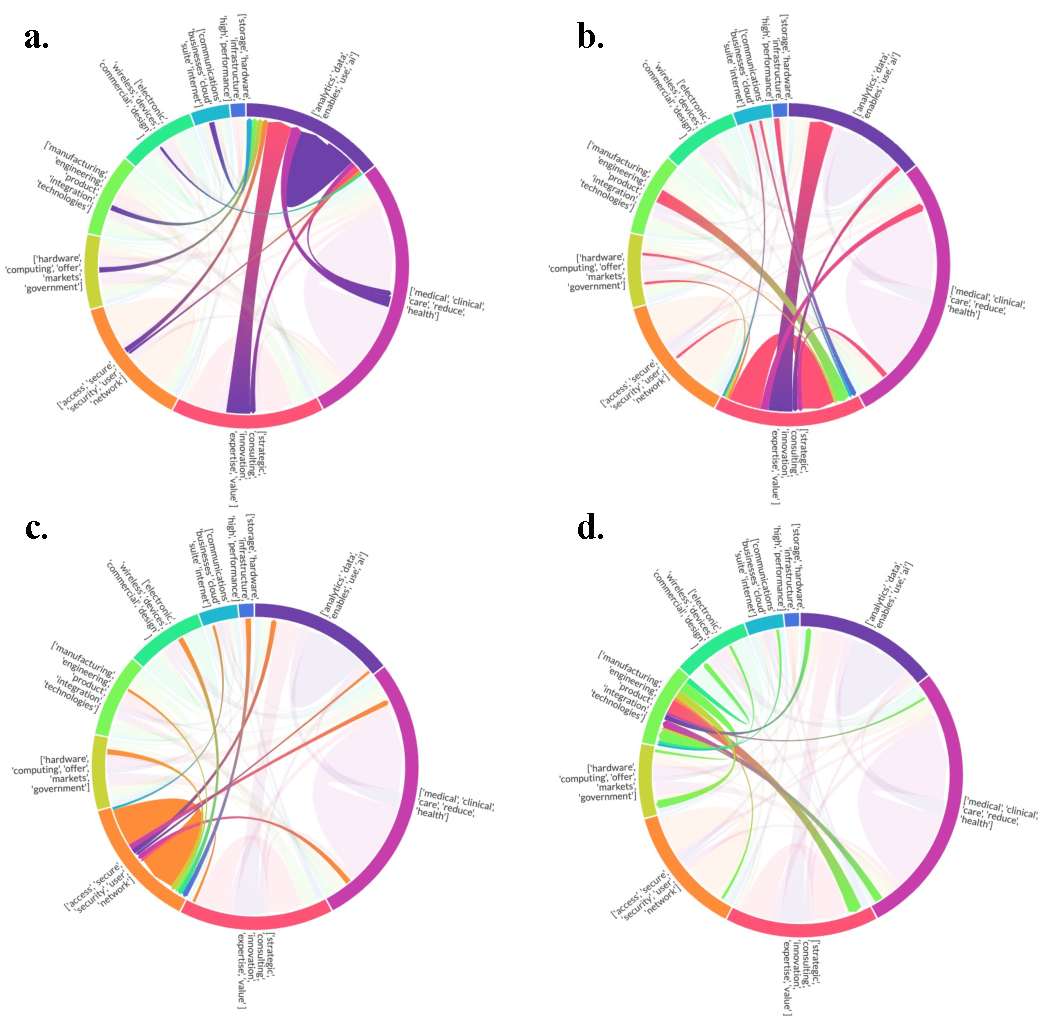
\includegraphics[width=0.95\textwidth]{5-5.pdf}
\caption{Visualizatio of value proposition transition. (a) 88\% increase in companies diversifying into data analytics and AI, (b) The number of companies focus on strategic and innovation consulting remains stable, but 33\% of these companies are also incorporating data analytics and AI into their services, (c) 32\% increase in companies expanding into access and network security, (d) 44\% decrease in companies primarily focusing on manufacturing.}
\label{fig:5-5}
\end{figure}

\subsubsection{Identify emerging value proposition trends in HPC adoption in healthcare over time}\label{subsec3.2.2}

In addition to observing the transition in value propositions for companies before and after HPC adoption, it is valuable to investigate the emerging trends of value propositions over time. To achieve this, we extract value propositions from all historical 10-k reports of companies operating in the healthcare sector that adopted HPC at certain years and employ topic modeling techniques. Figure~\ref{fig:5-6} highlights emerging trend-related topics such as novel oncology therapies, IoT, cybersecurity, and AI, as evidenced by the significant increase in the number of reports focusing on these topics since 2010. Furthermore, we identify companies associated with these emerging topics and analyze their performance over time. For instance, Merck \& Co., Inc. (CIK:310158), identified from the topic of novel oncology therapies, is one of the pioneers in computer-aided drug design since 1981 and has made significant investments in on-premises general purpose GPU technology in their strategy and roadmap~\cite{brown2017evolution}. Analysis of historical financial data from Compustat\footnote{\url{https://wrds-www.wharton.upenn.edu/pages/get-data/compustat-capital-iq-standard-poors/}} reveals that Merck's net profit margin (NPM) increased significantly to 21\% in 2019, with a return on investment (ROI) of 19\%. Furthermore, NPM increased to 25\% and 24\% in 2021 and 2022, respectively, while ROI remained stable around 18\% and 19\%. Additionally, Merck's stock price rose from \$23 in 2010 to \$130 in 2024. Ontrak, Inc. (CIK:1136174), an AI-powered and telehealth-enabled healthcare company specializing in personalized care programs, has experienced significant revenue growth since 2018, with growth rates of 97\%, 131\%, and 136\% in 2018, 2019, and 2020, respectively, indicating substantial business expansion. Similarly, DIGI INTERNATIONAL INC (CIK:854775), a leading global provider of business and mission-critical IoT connectivity products, contributes to enhanced patient outcomes and hospital operations through its provision of resilient and secure wireless connectivity. Since 2018, the company has maintained an average revenue growth rate of 16\%, accompanied by a steady increase in stock price from \$9.6 to \$32.6 since 2010. These positive company financial performances corroborate the role of HPC in facilitating shifts in novel value propositions and accelerating business growth.

\begin{figure}[!h]
\centering
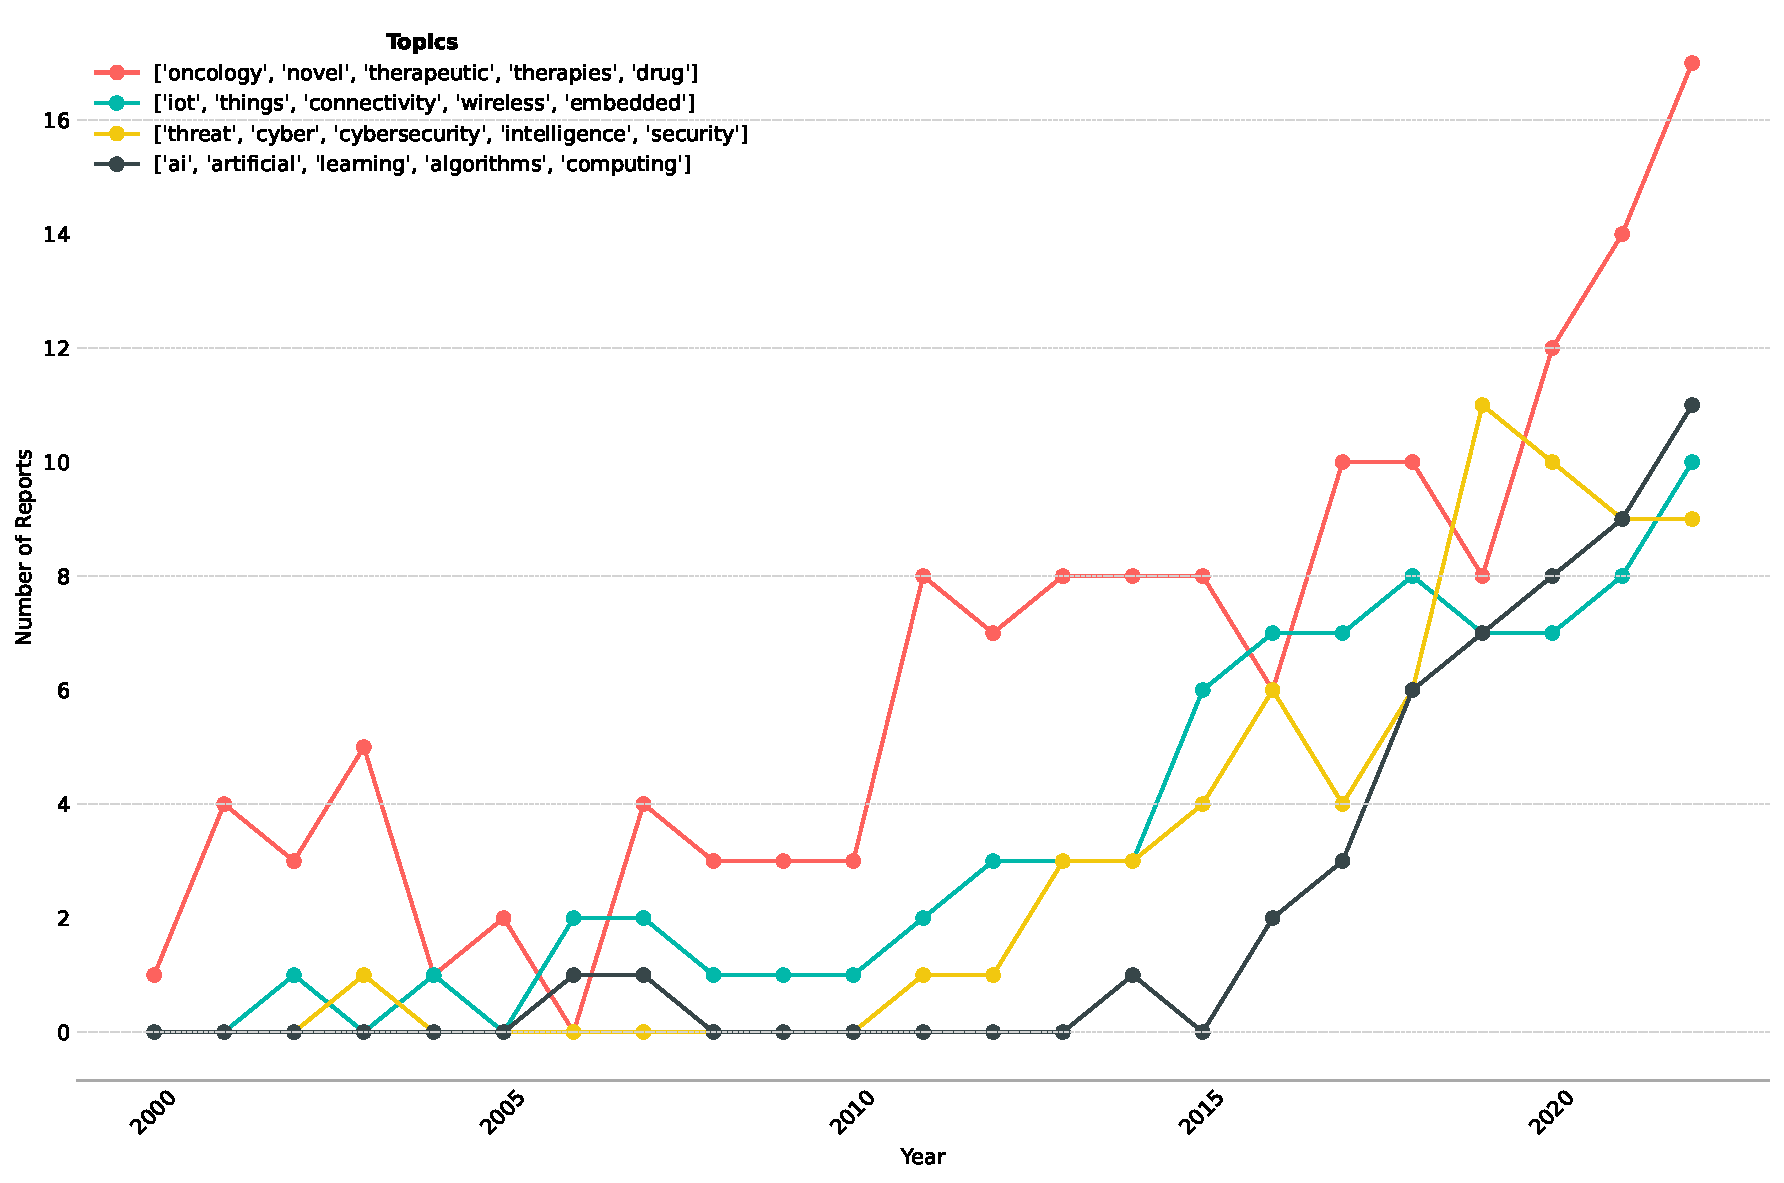
\includegraphics[width=0.95\textwidth]{5-6.pdf}
\caption{Line graph illustrating emerging trends of value proposition in HPC adoption in healthcare over time.}
\label{fig:5-6}
\end{figure}

\subsection{Customer segmentation transition}\label{subsec3.3}

HPC also substantially transforms approaches to customer segmentation, indicating a strategic shift towards diversification and expansion of customer bases. An impressive 85\% increase in companies targeting their services directly to patients underscores a transition towards a more patient-centric approach(panel (a) of Figure~\ref{fig:5-7}). This shift reflects a broader industry trend towards personalized healthcare, where advanced computing capabilities enable more tailored and efficient patient care solutions. Moreover, there's an 80\% rise in companies engaging with Small and Medium Enterprises (SMEs), indicating an expansion into serving businesses that are integral to the healthcare ecosystem, possibly through specialized services or technologies (panel (b) of Figure~\ref{fig:5-7}). About 41\% more companies have also started targeting organizations in the financial and insurance sectors related to life sciences (panel (c) of Figure~\ref{fig:5-7}), reflecting a strategic initiative to address the comprehensive needs of the healthcare industry, including financing and risk management. Additionally, the expansion into government and federal agencies, with a 20\% increase in companies targeting this segment (panel (d) of Figure~\ref{fig:5-7}), suggests a response to the growing opportunities in public health initiatives and regulatory compliance solutions.

\begin{figure}[!h]
\centering
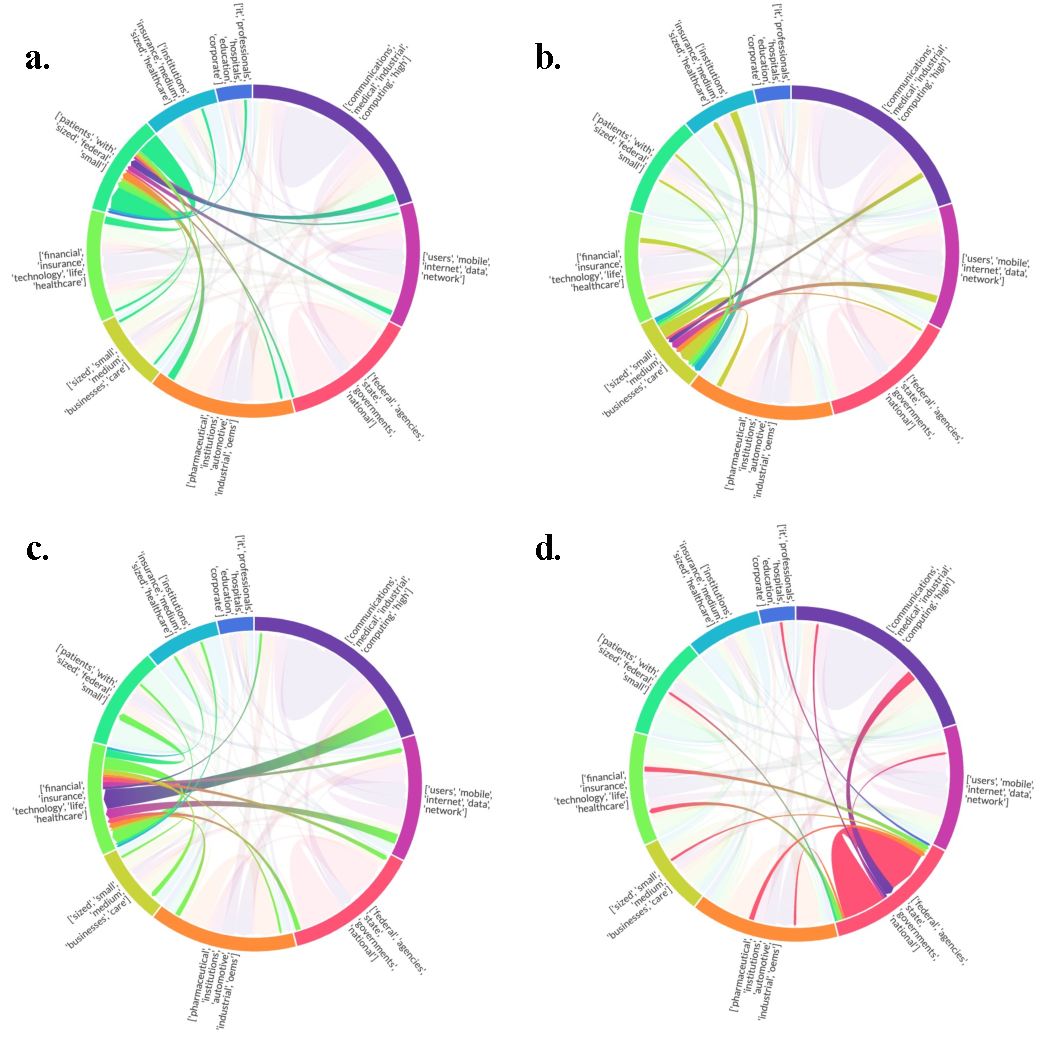
\includegraphics[width=0.95\textwidth]{5-7.pdf}
\caption{Visualizatio of customer segment transition. (a) 85\% increase in companies expanding their customer base directly to patients, (b) The number of company expanded their customer segment to SMEs increased  80\% (c) 41\% more companies catering to specialized sectors such as organizations operating in the financial, insurance relate to life sciences (d) 20\% increase in companies expanding their customer base to government/federal agencies.}
\label{fig:5-7}
\end{figure}

\subsection{Revenue stream transition}\label{subsec3.4}

Following the exploration of customer segment shifts, the landscape of revenue streams for healthcare companies reveals a significant evolution post-HPC adoption. This evolution marks a deliberate move towards more innovative and resilient financial models. The adoption of cloud computing has notably surged, evidenced by a 107\% increase in companies deriving their main revenue from cloud systems sales and maintenance (panel (a) of Figure~\ref{fig:5-8}). This trend highlights a strategic embrace of cloud computing's flexibility and scalability, crucial for managing the extensive data demands of modern healthcare. Furthermore, a 67\% rise in firms adopting subscription models underscores a growing preference for steady, recurring revenue streams (panel (b) of Figure~\ref{fig:5-8}). This shift towards subscription-based services reflects the sector's need for financial stability and continuous service enhancement, enabled by the ongoing advancements in HPC. The decrease in reliance on government and federal funding, with a 24\% drop in companies primarily funded by such means, suggests a strategic pivot towards the private sector and more diversified revenue sources (panel (c) of Figure~\ref{fig:5-8}). This movement is indicative of a broader desire to capitalize on the opportunities presented by HPC, steering away from traditional, less flexible funding models towards more dynamic and sustainable financial frameworks.

\begin{figure}[!h]
\centering
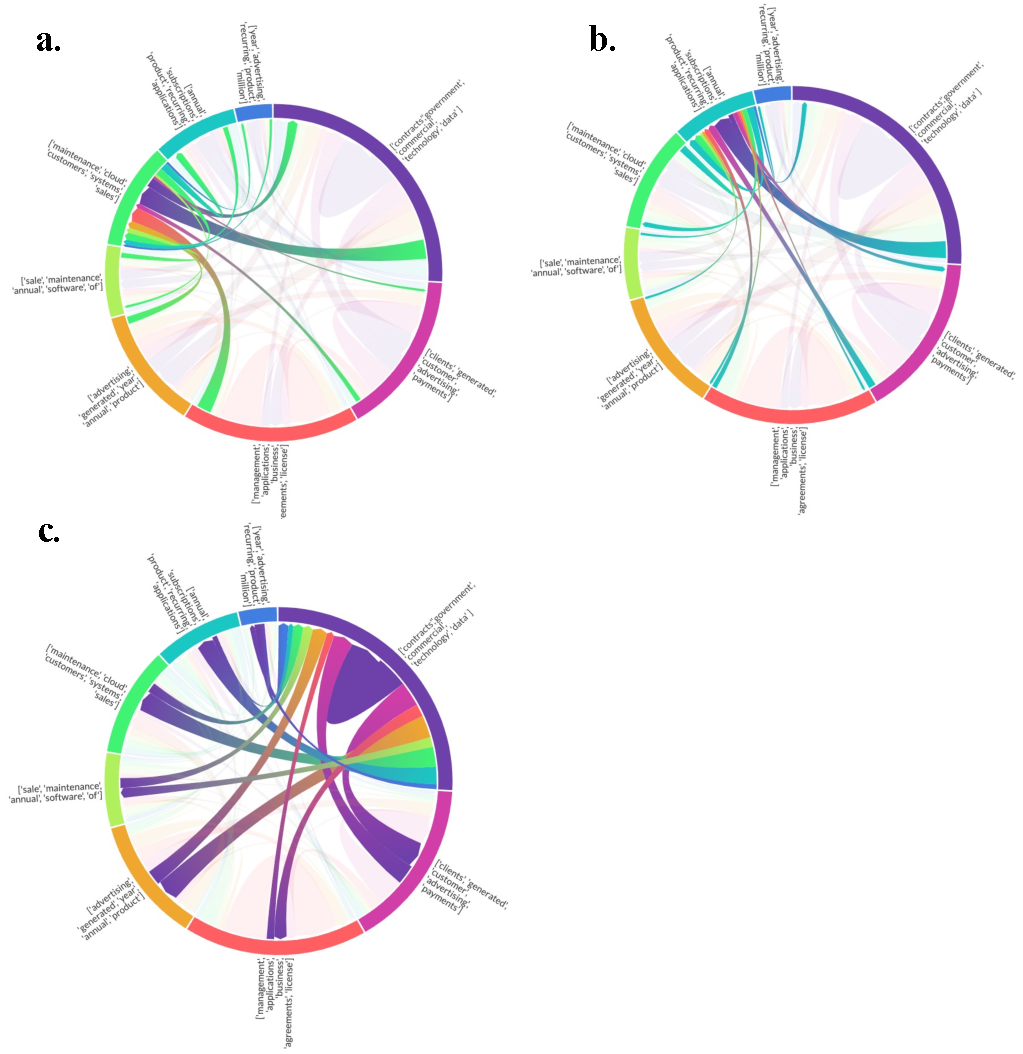
\includegraphics[width=0.95\textwidth]{5-8.pdf}
\caption{Visualization of revenue stream transition. (a) 107\% increase in the number of companies with main revenue stream from cloud systems sales/maintenance, (b) 67\% increase in the number of companies with main revenue stream from application subscriptions, (c) 24\% decrease in the number of companies with main revenue stream from government and federal agencies. }
\label{fig:5-8}
\end{figure}

\subsection{Cost structure transition}\label{subsec3.5}

In terms of cost structure perspective, a notable 47\% increase in operational costs reflects the substantial investments companies are making to refine their business models and enhance operations (panel (a) of Figure~\ref{fig:5-9}). These investments, while elevating short-term expenses, are aimed at harnessing the power of HPC for more efficient data processing and improved healthcare outcomes. Additionally, there's a 28\% rise in expenses related to data management and regulatory compliance (panel (b) of Figure~\ref{fig:5-9}), highlighting the complexities and costs associated with handling and securing large volumes of health data in an increasingly regulated environment.

Conversely, a 50\% reduction in manufacturing-related costs aligns with a strategic departure from traditional manufacturing towards more digital and service-oriented models (panel (c) of Figure~\ref{fig:5-9}). The shift away from manufacturing underscores a wider industry trend towards digital solutions and services, which, although lowering manufacturing costs, requires new investments in technological infrastructure and capabilities.

\begin{figure}[!h]
\centering
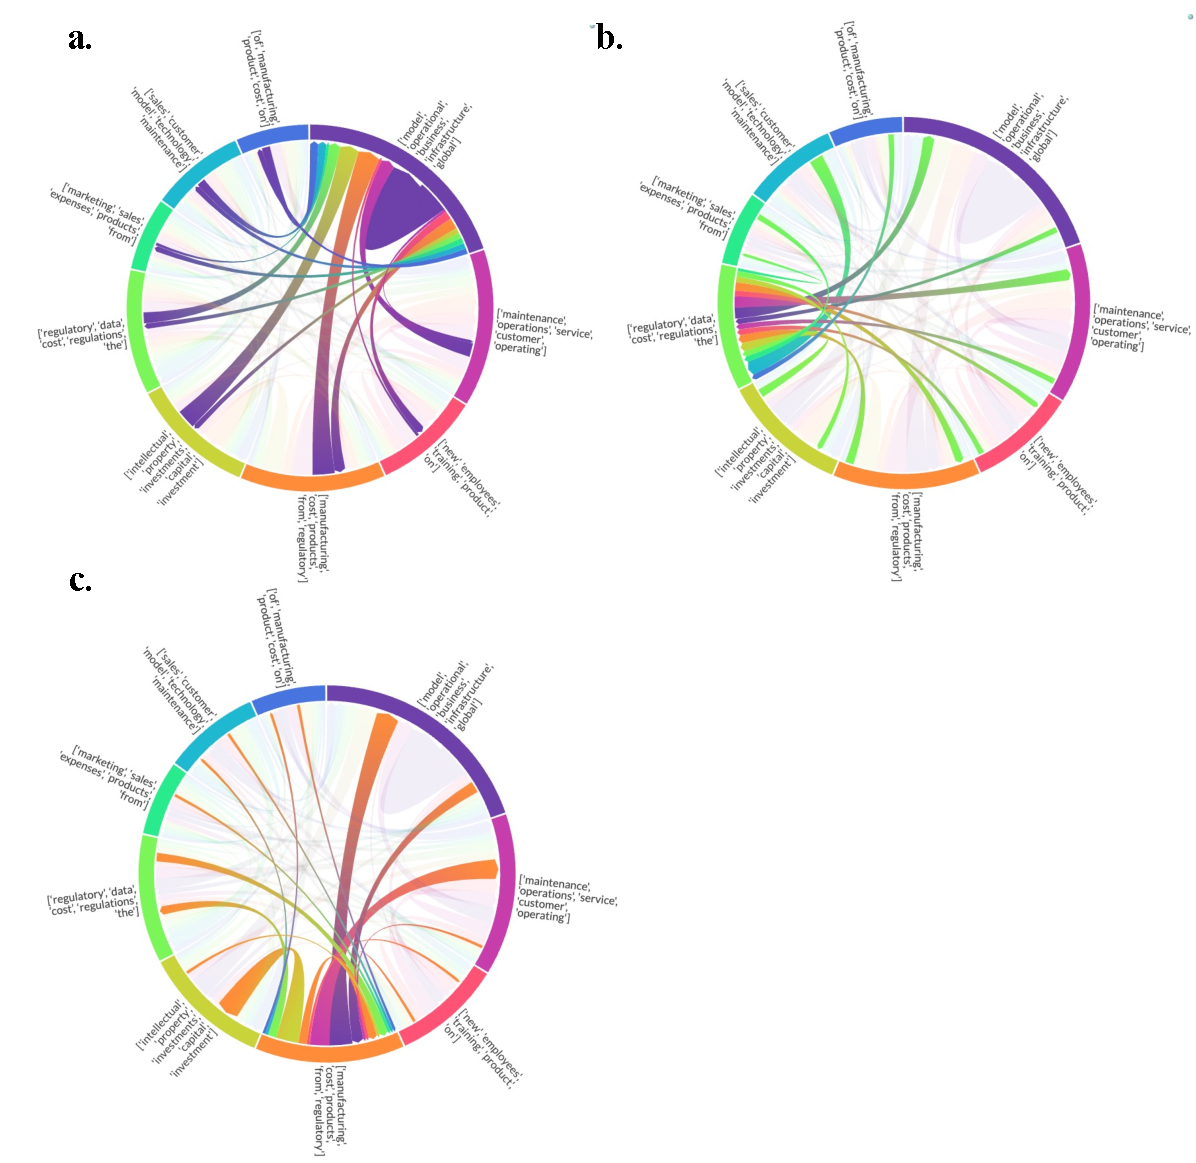
\includegraphics[width=0.95\textwidth]{5-9.pdf}
\caption{Visualization of cost structure transition. (a) 47\% increase in the number of companies whose primary cost structure is associated with business model refinement and operations, (b) 28\% increase in the number of companies whose primary cost structure is associated with data and regulation management. (c) 50\% decrease in the number of companies whose primary cost structure is associated with manufacturing.}
\label{fig:5-9}
\end{figure}

\subsection{Key activities  transition}\label{subsec3.6}

A significant observation is the 56\% increase in companies focusing on strategic technology implementation (panel (a) of Figure~\ref{fig:5-10}). This surge underscores the healthcare sector's recognition of the critical role technology plays in maintaining competitive advantage and addressing the complex challenges of modern healthcare delivery. Companies are investing more in integrating sophisticated technologies, such as HPC, to enhance their operational efficiency, data analytics capabilities, and ultimately, patient care services. Furthermore, there's been a 38\% increase in the emphasis on providing high-tech solutions and applications (panel (b) of Figure~\ref{fig:5-10}). This reflects a response to the healthcare industry's rapidly evolving technological needs, where there's a growing demand for advanced solutions that can process large volumes of data, support complex simulations, and deliver personalized patient care. The focus on high-tech solutions signifies a broader industry trend towards innovation and the adoption of cutting-edge technologies to meet the sophisticated needs of healthcare providers and patients alike.

\begin{figure}[!h]
\centering
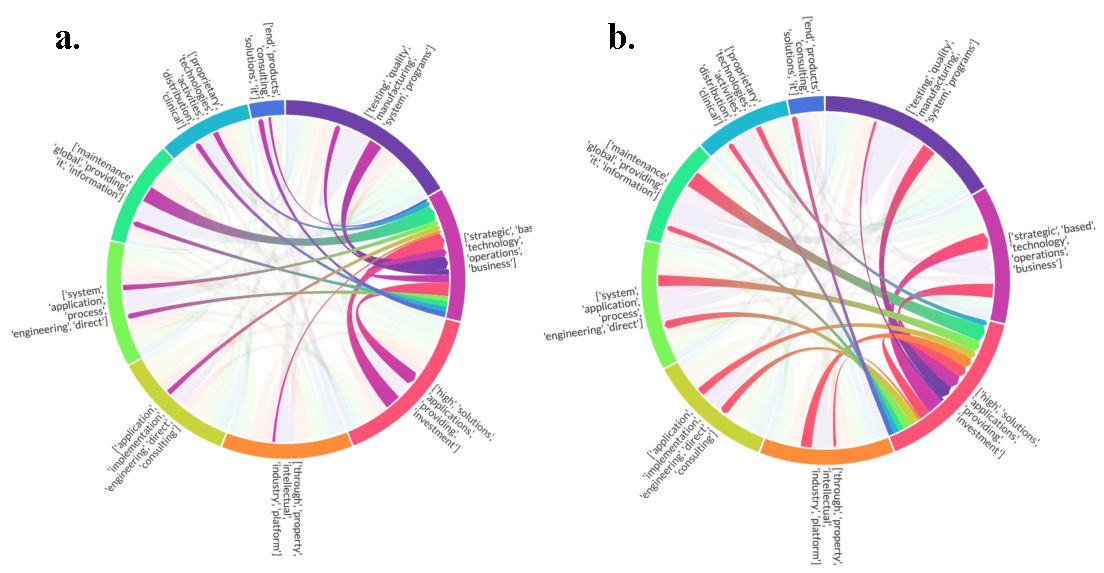
\includegraphics[width=0.95\textwidth]{5-10.pdf}
\caption{Visualization of key activities transition. (a) The number of company focus on strategic technology Implementation increased around 56\%, (b) 38\% increase in focus on providing high tech solutions.}
\label{fig:5-10}
\end{figure}

\subsection{Key resources  transition}\label{subsec3.7}

In terms of key resource perspective. a notable 42\% increase in companies identifying hardware and analytics tools as vital resources  (panel (a) of Figure~\ref{fig:5-11}), signifying the critical role of technological infrastructure in enabling data-driven healthcare solutions. This adjustment reflects a broader industry movement towards using computational power and analytical capabilities to process vast datasets. Moreover, the valuation of data as a key resource has escalated by 60\% (panel (b) of Figure~\ref{fig:5-11}), demonstrating the healthcare sector's increasing acknowledgment of data's essential role in enhancing care, advancing research, and encouraging innovation. This evolution emphasizes the strategic significance of data management and analysis capabilities.

Additionally, the changing dynamics around intellectual property, with a 29\% decline in the emphasis on trademarks and patents contrasted with a 13\% uptick in the valuation of other intellectual properties like product portfolios (panel (c and d) of Figure~\ref{fig:5-11}), indicate a nuanced shift in protecting and leveraging innovations. This evolution suggests a strategic realignment towards a broader conception of intellectual property, valuing comprehensive solutions and services that are increasingly vital in a technologically advanced healthcare ecosystem.

\begin{figure}[!h]
\centering
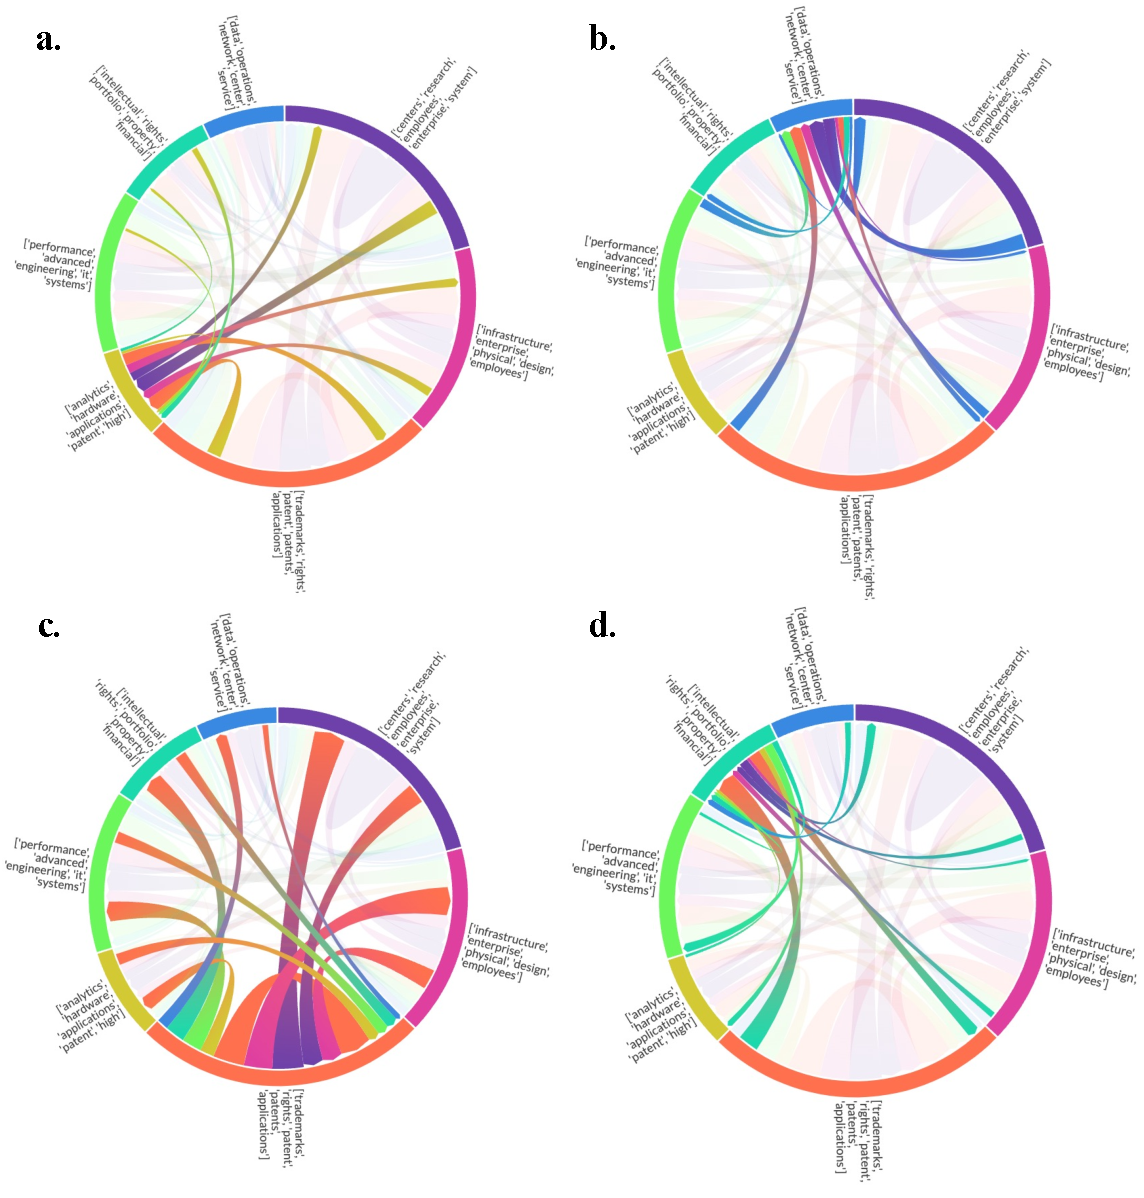
\includegraphics[width=0.95\textwidth]{5-11.pdf}
\caption{Visualization of key resources transition. (a) 42\% increase in companies treating hardware and analytics applications as key resources, (b) 60\% increase in valuing data as a key resources, (c) 29\% decrease in prioritizing trademarks and patents as key resources, (d) 13\% increase in valuing other intellectual properties like product portfolios as key resources.}
\label{fig:5-11}
\end{figure}


\section{Learning from the impact of HPC on business models in healthcare and identifying future opportunities}\label{sec4}

The ongoing business model transition within the healthcare industry is fundamentally a response to the technological revolution and the imperative to meet the evolving demands of healthcare delivery. The infusion of High-Performance Computing (HPC) is one of the catalysts for this shift, which is redefining the operational, strategic, and competitive landscape of healthcare businesses. This transition is characterized by a holistic shift towards technology and data-driven models, as evidenced by the industry's adoption of AI, data analytics, and cloud computing. These technological advancements have catalyzed a patient-centric approach, with healthcare companies broadening their market scope to engage directly with patients and diversifying their customer base. This strategic pivot is reshaping the operational framework and also redefining the nature of key resources, where the emphasis has shifted from physical assets to the valorization of data and intellectual property. The trend towards recurring revenue models is indicative of this transformation, reflecting a move away from traditional reliance on government funding and contracts towards more sustainable and predictable income streams. This technological shift is occurring because it aligns with broader trends of digitization and datafication that characterize contemporary economic and social environments. Businesses are compelled to transition not only due to the intrinsic benefits of technology but also to stay in step with these macro trends.

This transition is rooted in the pressing need for healthcare systems to become more efficient, cost-effective, and tailored to individual patient needs. Traditional models, heavily reliant on one-size-fits-all approaches and non-recurring revenue streams, are becoming obsolete in the face of personalized medicine and continuous care paradigms. Moreover, the push towards value over volume in healthcare reimbursement models encourages companies to invest in technologies that enhance patient outcomes and streamline operations. The evolution of revenue streams away from government or contract funding towards more predictable and stable sources underscores this strategic shift.

Looking forward, the incorporation of HPC is ready to unlock substantial opportunities for the healthcare industry. The shift from a one-time transactional model to ongoing, service-based relationships offers a platform for continuous innovation and improvement in patient care. Companies stand to gain from the development of new, data-centric business models that can adapt to and anticipate patient needs more effectively. Furthermore, as operational strategies lean more heavily on strategic technology investments, the potential for cross-sector collaborations and partnerships grows, potentially leading to a more integrated and efficient healthcare ecosystem. Protecting the increased volumes of sensitive data will also stimulate the growth of ancillary industries focused on cybersecurity and compliance, ensuring that the future of healthcare is not only technologically advanced but also secure and patient-focused.

\section{Discussion}\label{sec5}

In this study, we developed an automatic business model analysis framework by utilizing cutting-edge technologies such as LLM and the topic modeling technique Top2Vec. We applied this framework to analyze the impact of HPC on the business model transitions of companies in the healthcare domain, based on thousands of business reports. The interactive chord diagrams illustrate complex many-to-many relationships and transitions in an intuitive manner. This adaptable pipeline can be generalized to other domains by modifying the business report retrieval rules and will be beneficial for tracking and analyzing rapidly growing industries.

Due to the fact that 10-K reports are filed by all publicly traded companies within the United States, although many European or Asian-based companies are listed on U.S. stock exchanges, our analysis might potentially miss some entities operating in the HPC and healthcare-related domains. Secondly, our extraction of the BMC focuses on the business section (Item 1) of the 10-K report, as this section provides a comprehensive narrative of a company's ongoing operations and strategic directions. Its consistent and relevant data make it an ideal source for our analysis. Although other sections of the 10-K reports could also hold valuable information relate to business model, extracting the BMC from the entirety of thousands of 10-K reports using the GPT-4 model would be prohibitively costly and time-consuming. Consequently, our analysis concentrates on the business section of the 10-K reports.

One limitation of using topic models, like Top2Vec, is the need for human intervention to decide the optimal number of topics. This decision is subjective, relying on the analysis's specific context and objectives. The goal is to strike a balance between capturing the data's essential themes without creating too much overlap or too many divisions among topics. Thus, human insight and judgment are crucial in determining the right number of topics. To aid in this process, we utilize a dendrogram, which offers a more intuitive way to identify the ideal topic count.


Another issue with topic modeling is its lack of semantic understanding. Although topic models excel at detecting patterns in words and documents, they do not grasp the meanings behind the words. This shortfall can result in topics that are semantically inconsistent or challenging to interpret, necessitating manual review. One strategy to address this is through Entity Linking (EL), which adds a layer of explainability to topic modeling by connecting entities to a knowledge base, thereby enhancing topic interpretability~\cite{dillan2023ldaviewer,10.1145/3126686.3126776}. EL clarifies ambiguities by distinguishing between identical names referring to different entities, thus sharpening the accuracy of topic clusters. However, despite the assistance topic modeling provides in sifting through extensive business reports, it cannot replicate the nuanced and contextual insights provided by researchers. It should be regarded as a supportive tool rather than a replacement for the detailed exploration of business models. Acknowledging these limitations, future research should focus on refining this method, improving topic interpretability, and investigating alternative evaluation techniques. Despite its challenges, topic modeling continues to be an invaluable asset for comprehending the expanding corpus of business reports.

In conclusion, we introduce an innovative automated framework for analyzing business reports, aimed at understanding the impact of HPC on the evolutionary pathways of business models within the healthcare sector. Our framework encompasses the entire process, from retrieving and analyzing business reports to generating visual representations that illustrate the evolution of business models from various perspectives, utilizing the BMC. This adaptable framework can be tailored to suit different industries by adjusting the rules for retrieving business reports. Through the implementation of this automated analysis framework, we examined the trends in business model evolution among companies in the healthcare sector adopting HPC. These findings provide valuable insights for guiding future investments and the strategic advancement of HPC within the healthcare industry.


